\documentclass{article}
\usepackage[margin=1in]{geometry}
\usepackage{graphicx}
\usepackage{pdfpages}
\usepackage{hyperref}
\hypersetup{
    colorlinks=true,
    linkcolor=blue,
    filecolor=magenta,      
    urlcolor=cyan,
}
\usepackage{float}
\usepackage{caption}
\usepackage{subcaption}
\usepackage{array}
\usepackage{enumitem}

\title{CS M152A Lab 3: Finite State Machine - Vending Machine}
\author{Arnold Pfahnl \\ \small{TA: Mohit Garg, Winter 2021}}
\date{}

% \begin{figure}[H]
%     \centering
%     \includegraphics[scale=0.44]{../figs/.png}
%     \caption{}
%     \label{fig:}
% \end{figure}

\begin{document}
\maketitle
\tableofcontents

\section{Introduction}
In this lab, we implement a finite state machine used to operate a vending machine. The vending machine has $20$ unique two-decimal digit codes for different snacks. Each code represents a slot within which there can be up to $10$ units of a snack. This necessitates a counter for each slot. Other requirements include a buyer only being able to purchase $1$ item at a time, and card-only transactions.

The finite state machine is implemented in module $vending\_machine$. The inputs and outputs of the module are based on the following specifications in Table \ref{table:inputs} and Table \ref{table:outputs}, respectively.

\begin{table}[H]
    \centering
    \begin{tabular}{ | m{4cm} | m{8cm} | }
        \hline
        \textbf{Input} & \textbf{Size/Behavior} \\
        \hline
        $CLK$ & 100 MHz system clock. \\
        \hline
        $RESET$ & Synchronous reset signal. If high, item counters and outputs are set to $0$, and the machine enters the idle state. \\ 
        \hline
        $RELOAD$ & Reloads the machine by setting all counters to $10$. \\
        \hline
        $CARD\_IN$ & Signal that is high while the card is inserted into the machine. \\
        \hline
        $ITEM\_CODE[3:0]$ & The two-decimal digit item code input where each digit is entered one at a time. \\
        \hline
        $KEY\_PRESS$ & Indicates that $ITEM\_CODE$ is valid for reading when high. \\
        \hline
        $VALID\_TRAN$ & Indicates that the transaction using the card is valid when high. \\
        \hline 
        $DOOR\_OPEN$ & Indicates that the vending machine door is open when high. \\
        \hline
    \end{tabular}
    \caption{Inputs to $vending\_machine$ module.}
    \label{table:inputs}
\end{table}

\begin{table}[H]
    \centering
    \begin{tabular}{ | m{4cm} | m{8cm} | }
        \hline
        \textbf{Output} & \textbf{Size/Behavior} \\
        \hline
        $VEND$ & High when transaction is valid. Low when $DOOR\_OPEN$ goes high and then low or if the door doesn't open in 5 clock cycles. \\
        \hline
        $INVALID\_SEL$ & High if\dots \begin{enumerate}[noitemsep,topsep=0pt,]
            \item only 1 digit of $ITEM\_CODE$ entered and there is no second digit after $5$ clock cycles or if no digit is entered for $5$ clock cycles.
            \item the two-decimal digit $ITEM\_CODE$.
            \item the counter for on of the items is $0$.
        \end{enumerate} \\
        \hline
        $COST[2:0]$ & Once an item code is entered, this is set to the cost of that item and remains at this value until a new transaction begins. $000$ by default.  \\
        \hline
        $FAILED\_TRAN$ & High when signal doesn't go high within $5$ clock cycles of determining $ITEM\_CODE$. \\
        \hline
    \end{tabular}
    \caption{Outputs to $vending\_machine$ module.}
    \label{table:outputs}
\end{table}

The cost of each item based on the item code is depicted in Table \ref{table:costs} below.

\begin{table}[H]
    \centering
    \begin{tabular}{|c|c|}
        \hline
        \textbf{Item Code} & \textbf{Cost (\$)} \\
        \hline 
        00, 01, 02, 03 & 1 \\
        04, 05, 06, 07 & 2 \\
        08, 09, 10, 11 & 3 \\
        12, 13, 14, 15 & 4 \\
        16, 17 & 5 \\
        18, 19 & 6 \\
        \hline
    \end{tabular}
    \caption{Item costs in the $vending\_machine$ module.}
    \label{table:costs}
\end{table}

\section{Vending Machine Design}
The $vending\_machine$ module was created based on the finite state machine depicted in Figure \ref{fig:fsm}. There are seven main states: RESETTING, IDLE, RELOADING, CODE1, CODE2, TRANSACT, and VENDING.

\begin{enumerate}
    \item The \textbf{RESETTING} state can be transitioned to from any other state as long as RESET is high. In this state, all item counters and outputs are set to zero. When RESET becomes low, the machine transitions to the IDLE state.
    \item The \textbf{IDLE} state is the default state. When transitioning from another state to IDLE, all outputs are set to zero. The machine waits here until a new transaction is initiated with the CARD\_IN signal going high, transitioning to the CODE1 state. Alternatively, with the RELOAD signal, the machine can transition to the RELOADING state.
    \item The \textbf{RELOADING} state can only be accessed from the IDLE state with a RELOAD signal. In this state, all counters are set to 10, and the machine transitions back to IDLE when the RELOAD signal goes low.
    \item The \textbf{CODE1} state can only be accessed from the IDLE state with a CARD\_IN signal. In this state, we store the value of ITEM\_CODE as the first digit of the two-digit code when KEY\_PRESS goes high. In my implementation, the combination of KEY\_PRESS high and the code being stored is indicated by the CODE1\_STORED internal signal. Additionally, an internal INVALID\_SEL\_DETECT bit is set if this first digit is not valid. If a KEY\_PRESS is not detected in 5 cycles, INVALID\_SEL is set to high, and the machine transitions to the IDLE state.
    \item The \textbf{CODE2} state can only be accessed from the CODE1 state after the first digit has been stored. In this state, we store the value of ITEM\_CODE as the second digit of the two-digit code when KEY\_PRESS goes high. In my implementation, the combination of KEY\_PRESS high and the code being stored is indicated by the CODE2\_STORED internal signal. Additionally, the INVALID\_SEL\_DETECT bit is set if this second digit is not valid or if there are no items left for the item selected. If a KEY\_PRESS is not detected in 5 cycles, INVALID\_SEL is set to high, and the machine transitions to the IDLE state.
    \item The \textbf{TRANSACT} state can only be accessed from the CODE2 state after the second digit has been stored. 
    
    If the selection is determined to be invalid based on INVALID\_SEL\_DETECT being high, INVALID\_SEL is set to high and the machine transitions to the IDLE state.

    For a valid selection, the machine waits for the VALID\_TRAN signal to go high. If this doesn't happen within 5 clock cycles, the machine transitions to the IDLE state and FAILED\_TRAN is set to high. With VALID\_TRAN set to high, the machine transitions to the final state: VENDING.

    A valid selection also means that COST will be set to the dollar amount as specified by Table \ref{table:costs}. To determine the cost of an item, an internal function called $find\_cost$ takes the stored first digit and second digit as inputs, and determines the cost with a series of if-else statements. In pseudocode:
    \begin{verbatim}
        if the first digit is 0:
            if the second digit is in [0, 3]:
                return 1
            if the second digit is in [4, 7]:
                return 2
            otherwise return 3
        if the first digit is 1:
            if the second digit is in [0, 1]:
                return 3
            if the second digit is in [2, 5]:
                return 4
            if the second digit is in [6, 7]:
                return 5
            otherwise return 6
    \end{verbatim}

    \item The \textbf{VENDING} state can only be accessed from the TRANSACT state. In this state, the item that was selected has its counter decremented by one and VEND is set to high. Then the machine waits for the DOOR\_OPEN signal to go high and then low before transitioning to the IDLE state. The machine will transition to the IDLE state if the door doesn't open for 5 clock cycles. It's also worth noting that a little peculiarity with this state is that if the door stay open without closing, the machine will stay in this state until a door close or a reset.
\end{enumerate}

To take care of states that have a timeout condition, my implementation has a timer that starts when transitioning between different states. Regardless of whether or not a state will take advantage of the timer, the timer will increment by one every cycle until the state is in its fifth cycle at which point an internal TIMEOUT signal is set high. States that use a timer will recognize the TIMEOUT signal and transition as needed.

\begin{figure}[H]
    \centering
    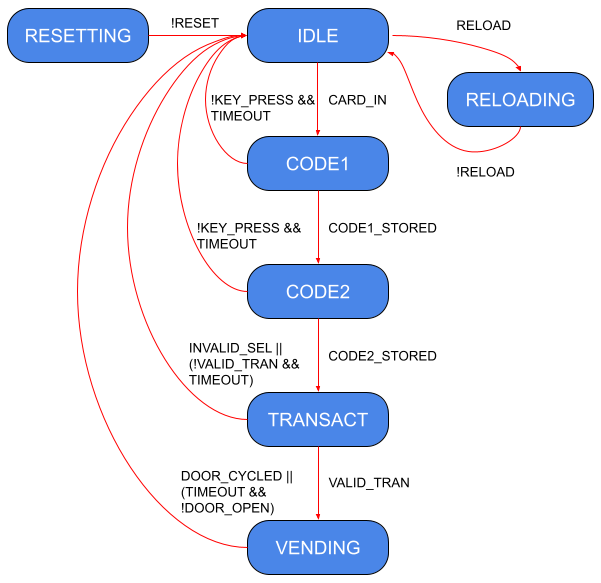
\includegraphics[scale=0.44]{../figs/FSM.png}
    \caption{Finite state machine flow chart for the $vending\_machine$ module.}
    \label{fig:fsm}
\end{figure}

\pagebreak
\subsection{Schematics}
The top level schematic in Figure \ref{fig:schem_top} hides the considerable complexity of the RTL schematic in Figure \ref{fig:schem_detailed}. Due to the combination of both combinational and sequential logic used to determine states and output, the RTL features a mess of registers, muxes, and many other gates. Notably, the long vertical line of registers on the left are for the counters. There are also large muxes used to determine item cost and state transitions.
\begin{figure}[H]
    \centering
    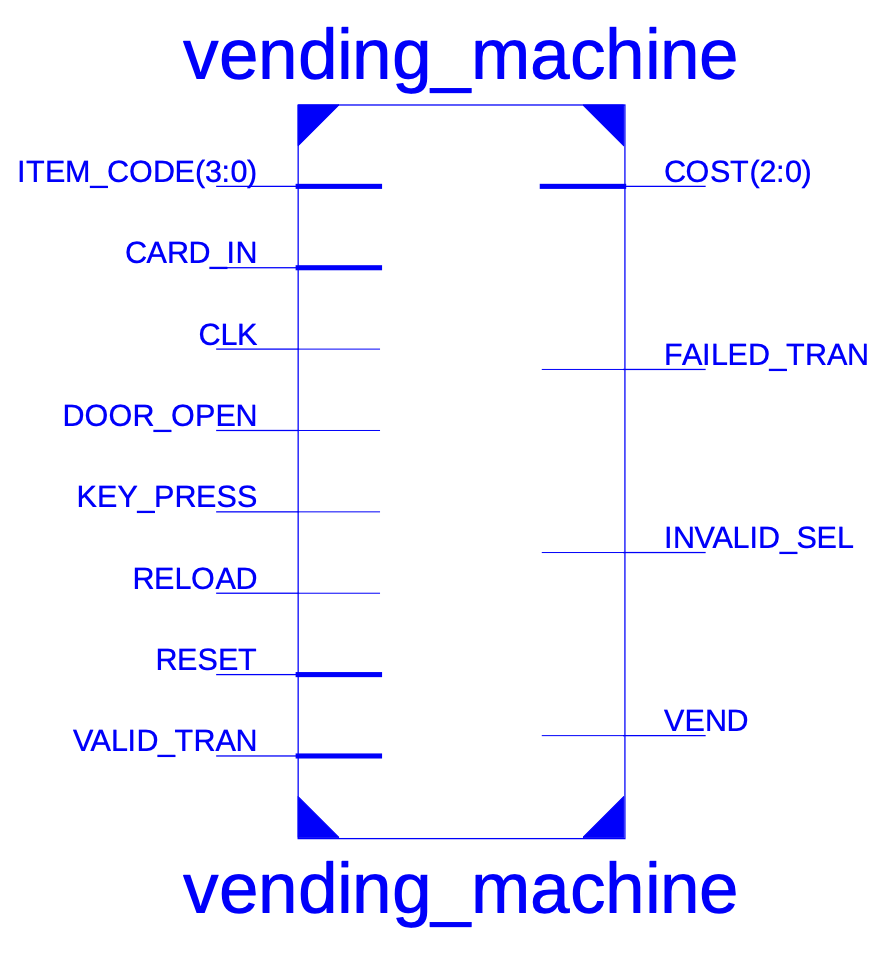
\includegraphics[scale=0.42]{../figs/schematic.png}
    \caption{Top level schematic for the $vending\_machine$ module.}
    \label{fig:schem_top}
\end{figure}

\begin{figure}[H]
    \centering
    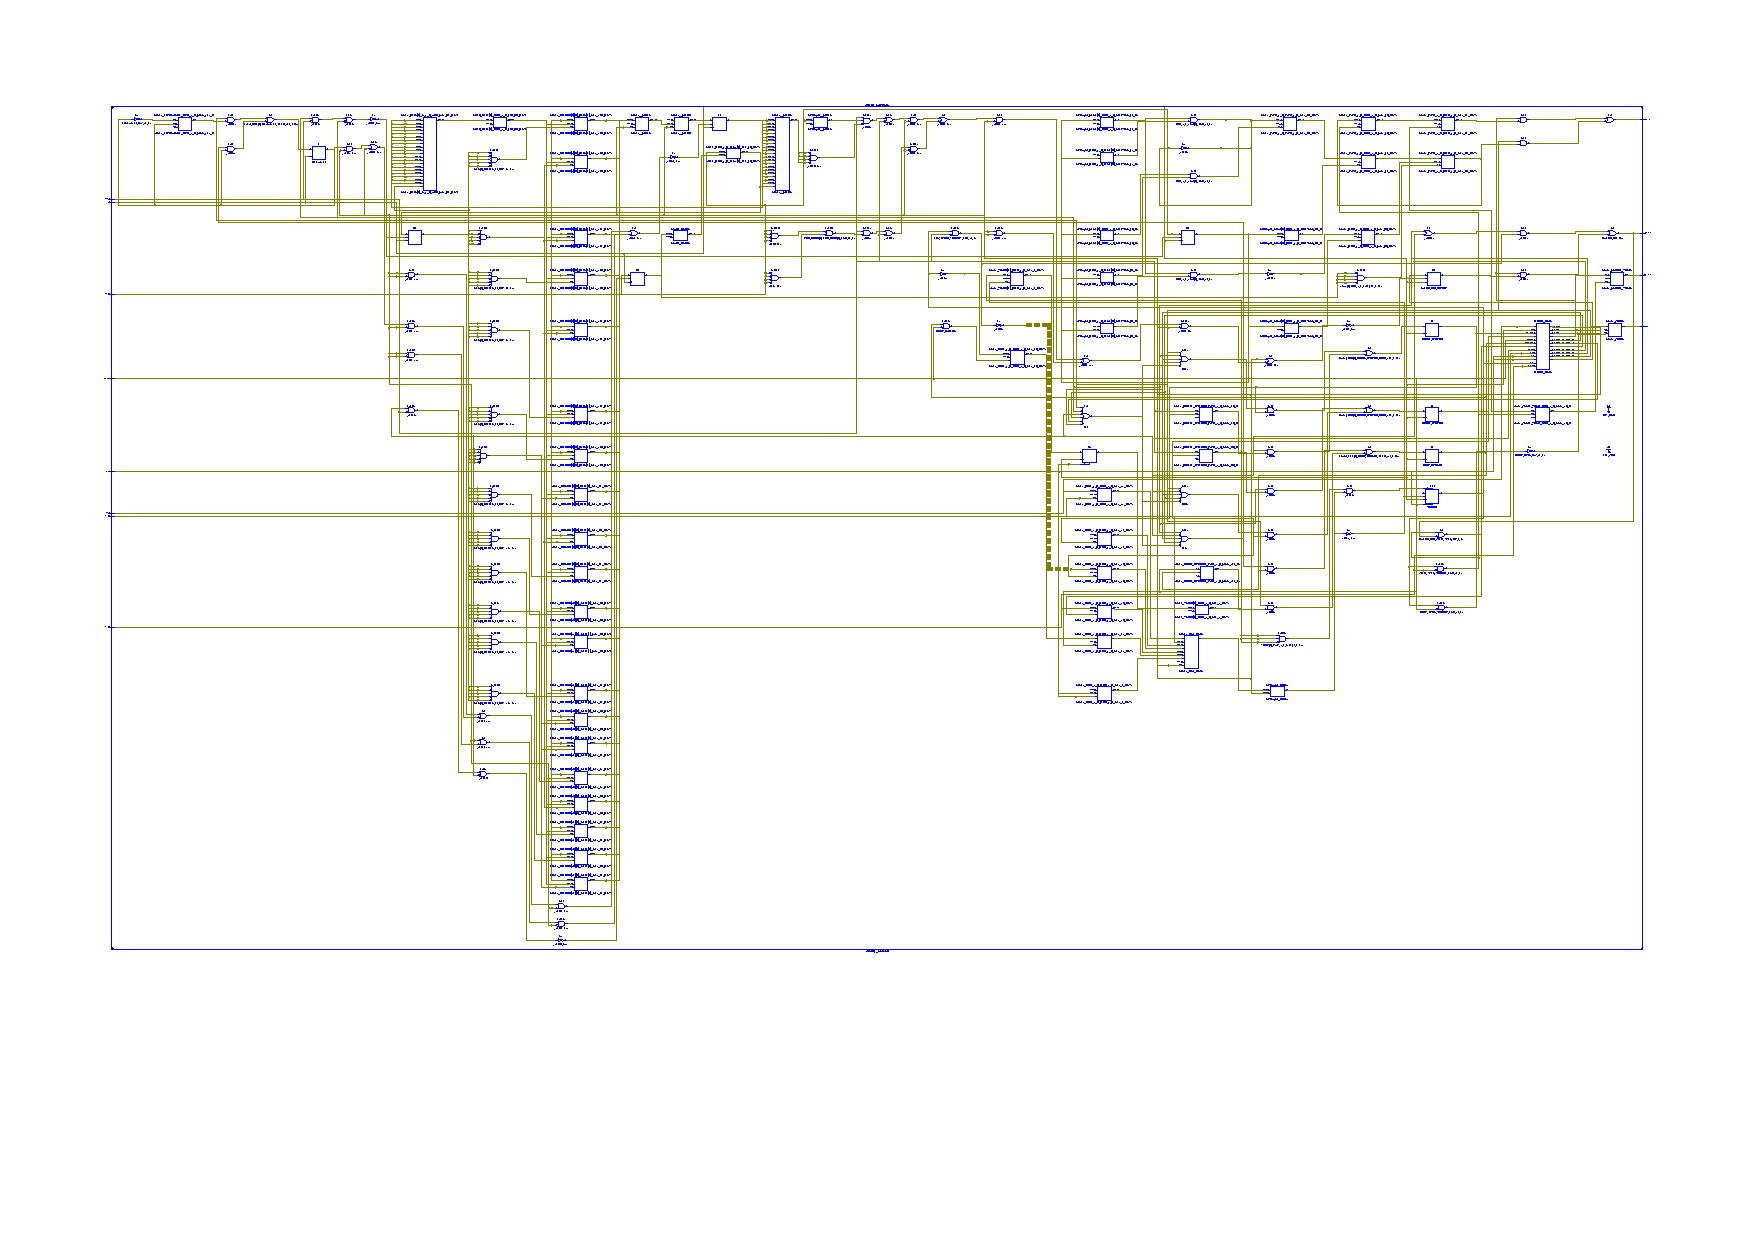
\includegraphics[scale=0.6]{../figs/schematic_detailed.pdf}
    \caption{Detailed RTL schematic for the $vending\_machine$ module.}
    \label{fig:schem_detailed}
\end{figure}

\subsection{Design Summary Report}

{\centering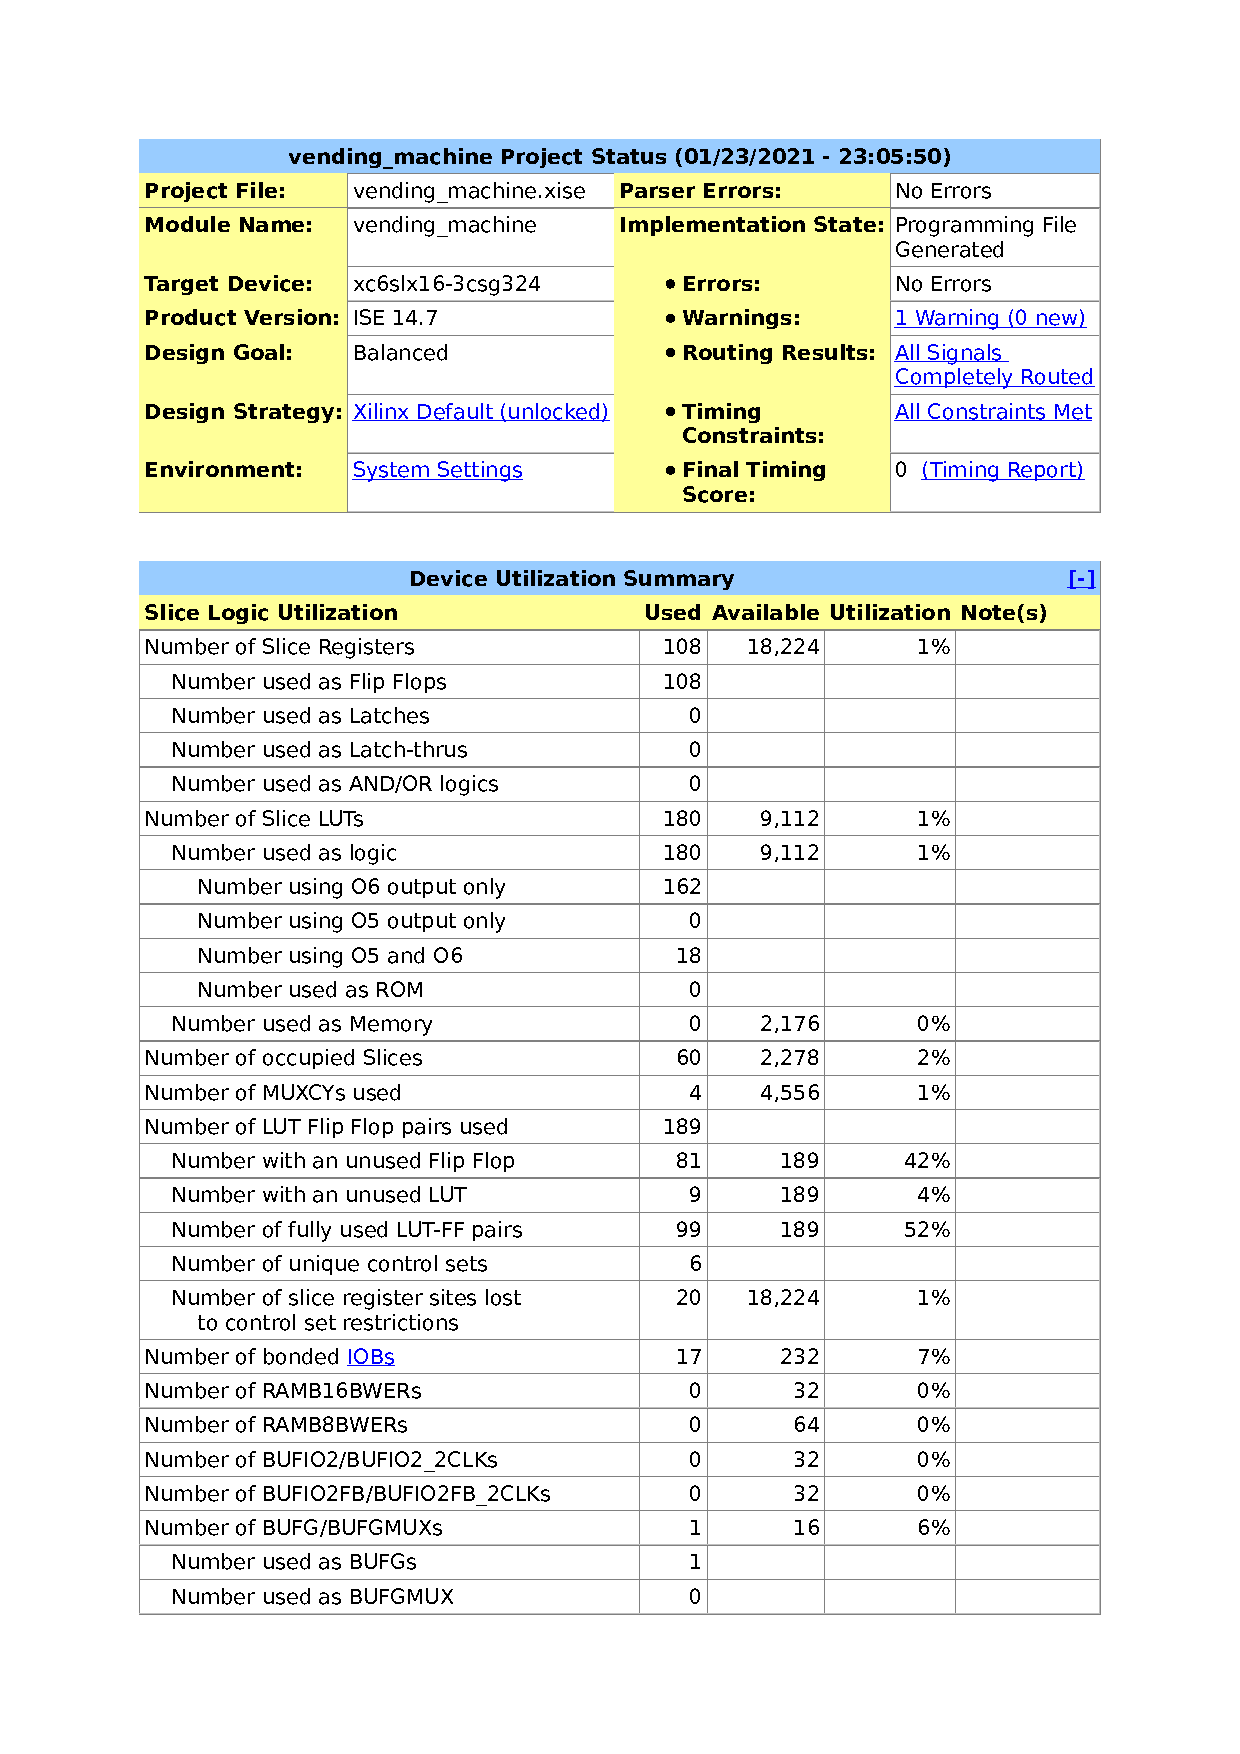
\includegraphics[scale=0.8, page=1]{../figs/design_summary.pdf}\par}

{\centering\includegraphics[scale=0.8, page=2]{../figs/design_summary.pdf}\par}

{\centering\includegraphics[scale=0.8, page=3]{../figs/design_summary.pdf}\par}

\pagebreak
\section{Simulation}

To test the $vending\_machine$ module, I created a few helper tasks. Task $reset\_in()$ resets all the inputs to the module to zero. Task $reset\_n\_load()$ calls $reset\_in$ and also transitions the machine from IDLE to RELOADING and back. Task $vend\_cycle()$ takes two digits representing a two-digit item code and runs through a full cycle. These three tasks help streamline the initialization and setup of multiple tests.

My tests also include a 100 MHz clock, CLK. To aid in testing, an always block offset by half a cycle prints out the errors for INVALID\_SEL and FAILED\_TRAN when the corresponding outputs go high. In general, inputs to the module are offset by half a cycle to prevent strange behavior happening.

The following is a description of the tests:
\begin{enumerate}
    \item \textbf{No reload.} The purpose of this test is to ensure that INVALID\_SEL is set when trying to vend an item that has a counter at 0, and that with no reload, the counters are indeed at 0. As expected INVALID\_SEL was set appropriately, and the machine transitioned back to the IDLE state. See Figure \ref{fig:sim1_2}.
    \item \textbf{Valid run.} This test does a full run of a valid vending cycle (no errors). This test establishes a baseline for making sure that the module can function at its most basic level. As expected, the test passed with no errors. See Figure \ref{fig:sim1_2}.
    \item \textbf{Full to empty slot.} This test makes sure that the vending machine vends properly, counters reach 0, and that an item will only be able to vend 10 times with only one reload. This test reloads the machine and vends the same item 12 times. As expected, the module vends 10 items and then sets INVALID\_SEL the last two times. See Figure \ref{fig:sim3}.
    \item \textbf{Invalid selection number.} This is a simple test that checks if an invalid selection will trigger INVALID\_SEL. Specifically $20$ was chosen, and this test passed as expected. See Figure \ref{fig:sim4_5}.
    \item \textbf{Key press timeout.} This test actually contains two tests in one. First, a vending cycle is started but then KEY\_PRESS is never set high for the first digit. This resulted in the machine returning to IDLE after 5 cycles as expected. Following the failed vend, another vending cycle is started, the first digit is entered successfully, but then the second digit times out. This resulted in the machine returning to IDLE as expected. See Figure \ref{fig:sim4_5}.
    \item \textbf{Door timeout.} This test checks to see if the machine will handle a door timeout properly. Once the VENDING state is reached, DOOR\_OPEN is never set high. In testing, the machine went back to the IDLE state after 5 cycles as expected. See Figure \ref{fig:sim6_7_8}.
    \item \textbf{Door open.} This is an edge case where the door stays open during the VENDING state. In this case, the machine ignored TIMEOUT and stayed in the VENDING state as required by the specifications. See Figure \ref{fig:sim6_7_8}.
    \item \textbf{Failed transaction.} This test simulates a failed transaction with the expectation that the machine sets FAILED\_TRAN and transitions back to IDLE. In testing, the machine passed this test as expected. See Figure \ref{fig:sim6_7_8}.
\end{enumerate}

\begin{figure}[H]
    \centering
    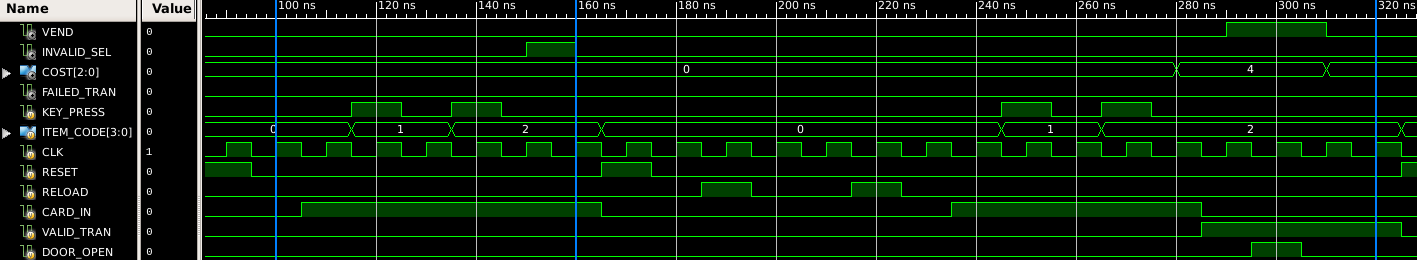
\includegraphics[scale=0.33]{../figs/sim1_2.png}
    \caption{No reload (100 to 160 ns) and valid run (160 to 320 ns) simulation waveforms. Item 12 is selected for the no reload test after which INVALID\_SEL is selected since the machine hasn't been loaded yet. The valid run ends with a successful vend and all outputs reset once the machine enters the IDLE state.}
    \label{fig:sim1_2}
\end{figure}

\begin{figure}[H]
    \centering
    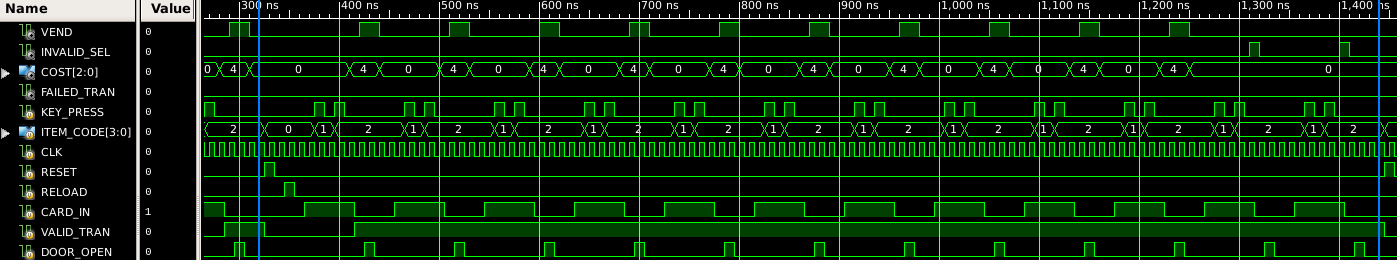
\includegraphics[scale=0.35]{../figs/sim3.png}
    \caption{Full to empty on item 12 simulation waveform. Note the 10 successful vends and the two invalid selections due to the slot being empty.}
    \label{fig:sim3}
\end{figure}

\begin{figure}[H]
    \centering
    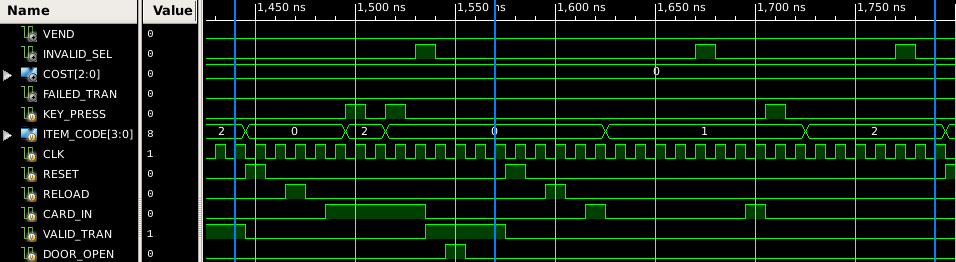
\includegraphics[scale=0.35]{../figs/sim4_5.png}
    \caption{Invalid selection number (1440 to 1570 ns) and key press timeout (1570 to 1790 ns) simulation waveforms. The invalid selection number used is 20. Note that for the key press timeout the first time INVALID\_SEL is high is 5 cycles after CARD\_IN is detected, and the second time INVALID\_SEL is high is 5 cycles after the first digit is processed (6 cycles after the first digit's KEY\_PRESS).}
    \label{fig:sim4_5}
\end{figure}

\begin{figure}[H]
    \centering
    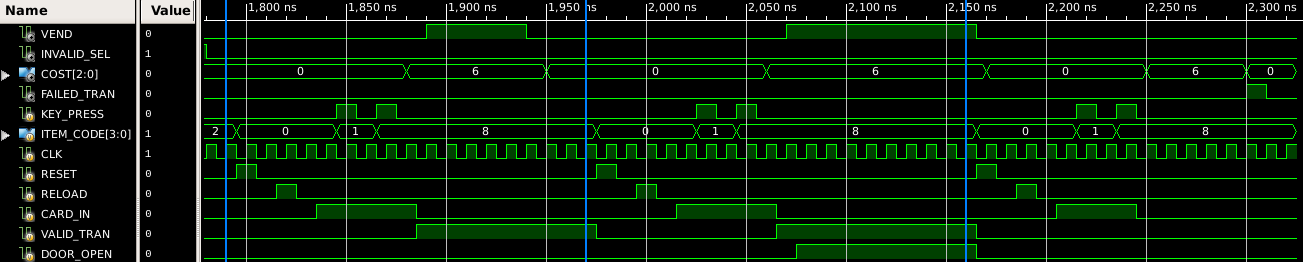
\includegraphics[scale=0.35]{../figs/sim6_7_8.png}
    \caption{Door timeout (1790 to 1970 ns), door open (1970 to 2160 ns), and failed transaction (2160 to 2320 ns). For door timeout, note how VEND is high for 5 cycles before being set to low. For door open, note how VEND is high even after 5 cycles since DOOR\_OPEN is stuck open. For failed transaction, note how FAILED\_TRAN is set high after 5 cycles without the VALID\_TRAN signal (6 cycles after saving the second digit in the CODE2 state).}
    \label{fig:sim6_7_8}
\end{figure}

\section{Conclusion}
In the lab, I was able to successfully create a finite state machine (FSM) that works as a vending machine. My FSM also handles some tougher edge cases confirmed by my testing. 

This lab was much more involved than previous labs; however, I found the material engaging and interesting, especially in terms of complex Verilog coding and FSMs as a concept.

I did find that some aspects of the vending machine specifications weren't entirely realistic, but given the complexity of the project as is, it makes sense to not have us worry about those conditions. In general, I thought the project was well put together, and I didn't run into too many issues.

\end{document}